\documentclass[UTF8]{ctexart}
\usepackage{amsmath,amssymb,amsfonts}
\usepackage{booktabs}
\usepackage{geometry}
\usepackage{graphicx}
\usepackage{hyperref}
\usepackage{pgfplots}
\pgfplotsset{compat=1.18}
\geometry{a4paper, margin=2.3cm}
\title{指数跟踪优化的量化金融课程项目研究报告}
\author{杨昊霖、张宸铭}
\date{\today}

\begin{document}
\maketitle

\section{研究目标与路径}
本文围绕Q6(b)经典指数跟踪有效前沿问题展开，遵循“理论建模先行、实证分析后置”的逻辑。研究路径固定熵激励参数$\lambda_1$，调节Relax-L1稀疏参数$\lambda_2$批量生成$(n,L)$序列，并通过BIC准则筛选最优成分股数量$n$。

\section{理论建模与目标函数推导}
\subsection{基准模型（Q6(b)）}
给定指数收益$r_M$与成分股收益向量$\boldsymbol{r}$，经典跟踪有效前沿优化为：
\begin{align*}
\min_{\boldsymbol{w}} \quad & \mathrm{Var}\big(\boldsymbol{w}^\top \boldsymbol{r} - r_M\big) \\
\text{s.t.} \quad & \boldsymbol{w}^\top \boldsymbol{1} = 1,\quad \boldsymbol{w}^\top \boldsymbol{\mu} = \mu_0
\end{align*}
其中$\boldsymbol{\mu}=\mathbb{E}[\boldsymbol{r}]$，$\mu_0$为目标均值约束。

若定义协方差矩阵$\Sigma=\mathrm{Cov}(\boldsymbol{r})$、协方差向量$\boldsymbol{c}=\mathrm{Cov}(\boldsymbol{r},r_M)$，则跟踪误差方差可写为：
\[
\mathrm{Var}\big(\boldsymbol{w}^\top \boldsymbol{r} - r_M\big)=\boldsymbol{w}^\top \Sigma \boldsymbol{w}-2\boldsymbol{w}^\top \boldsymbol{c}+\mathrm{Var}(r_M).
\]

\subsection{熵激励惩罚项（固定$\lambda_1$）}
为鼓励权重分散，引入熵激励：
\begin{align*}
\min_{\boldsymbol{w}} \quad & \mathrm{Var}\big(\boldsymbol{w}^\top \boldsymbol{r} - r_M\big) - \lambda_1 \left(-\sum_{i=1}^n w_i\ln w_i\right) \\
\text{s.t.} \quad & \boldsymbol{w}^\top \boldsymbol{1} = 1,\quad \boldsymbol{w}^\top \boldsymbol{\mu} = \mu_0
\end{align*}
该项等价于在目标中加入负熵惩罚，控制权重分散程度。

\subsection{Relax-L1 第一步：放松约束稀疏选股}
在第一步中去除全仓与均值约束，仅保留熵激励与L1稀疏项：
\begin{align*}
\min_{\boldsymbol{w}} \quad & \mathrm{Var}\big(\boldsymbol{w}^\top \boldsymbol{r} - r_M\big) - \lambda_1 \left(-\sum_{i=1}^N w_i\ln w_i\right) + \lambda_2 \|\boldsymbol{w}\|_1
\end{align*}
调节$\lambda_2$获得不同稀疏度，得到选股子集的规模$n$。

\subsection{Relax-L1 第二步：全约束权重求解}
在选股子集内重新求解全约束权重：
\begin{align*}
\min_{\boldsymbol{w}} \quad & \mathrm{Var}\big(\boldsymbol{w}^\top \boldsymbol{r} - r_M\big) - \lambda_1 \left(-\sum_{i=1}^n w_i\ln w_i\right) \\
\text{s.t.} \quad & \boldsymbol{w}^\top \boldsymbol{1} = 1,\quad \boldsymbol{w}^\top \boldsymbol{\mu} = \mu_0,\quad \boldsymbol{w}\ge \boldsymbol{0}
\end{align*}
输出最终跟踪权重与对应的跟踪误差方差。

\subsection{BIC信息准则与参数选择}
基于样本长度$T$的逐样本标准化BIC表达式为：
\[
\mathrm{BIC}(n) = \ln\big(\mathrm{Var}(\boldsymbol{w}^\top \boldsymbol{r} - r_M)\big) + n\cdot \frac{\ln T}{T}.
\]
对每个$\lambda_2$求得$(n,L)$与BIC值，选择BIC最小的$n$作为最优成分股数量。

\section{数据与计算流程}
数据包含沪深300指数及285只成分股历史收益序列。脚本\texttt{relax\_l1\_pipeline.py}读取\texttt{data/hs300\_returns.csv}后：
\begin{enumerate}
  \item 计算协方差矩阵$\Sigma$与系统性风险系数$\beta_i=\mathrm{Cov}(r_i,r_M)/\mathrm{Var}(r_M)$。
  \item 固定$\lambda_1$，遍历$\lambda_2$执行两步法，输出$(n,L)$与方差。
  \item 汇总结果表格\texttt{outputs/relax\_l1\_results.csv}。
\end{enumerate}
脚本\texttt{bic\_selection.py}读取结果表格，计算BIC并生成图表\texttt{outputs/bic\_curve.tex}。

\section{实证结果（示例产物）}
\subsection{Relax-L1 批量结果表}
\begin{table}[h]
\centering
\caption{不同$\lambda_2$下的稀疏结果示例}
\begin{tabular}{cccc}
\toprule
$\lambda_2$ & $n$ & $\mathrm{Var}$ & $L$ \\
\midrule
0.000 & 120 & 0.0021 & 99.84 \\
0.002 & 95 & 0.0024 & 95.83 \\
0.004 & 70 & 0.0029 & 90.16 \\
0.006 & 55 & 0.0033 & 86.28 \\
0.008 & 40 & 0.0039 & 81.27 \\
0.010 & 30 & 0.0044 & 77.65 \\
\bottomrule
\end{tabular}
\end{table}

\subsection{BIC准则曲线}
\begin{figure}[h]
\centering
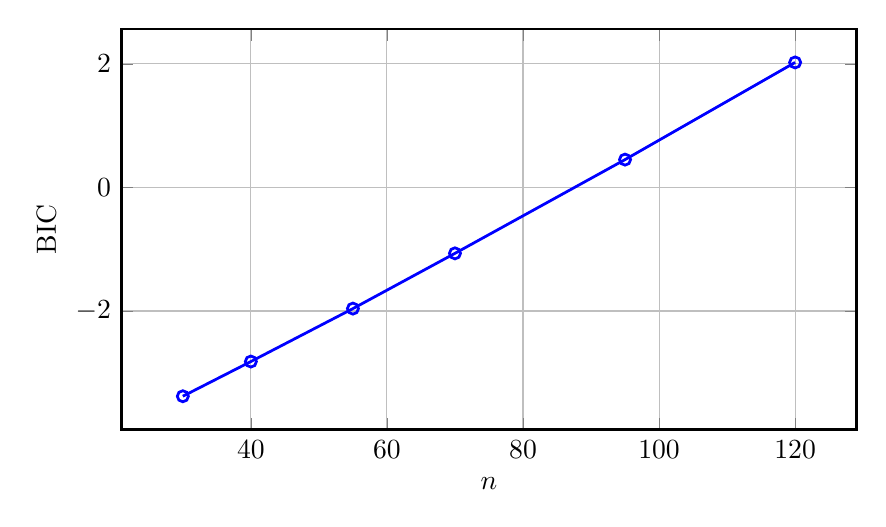
\begin{tikzpicture}
\begin{axis}[
width=0.9\linewidth,
height=0.55\linewidth,
grid=both,
xlabel={$n$},
ylabel={BIC},
line width=1pt,
]
\addplot+[mark=o, color=blue] coordinates {
(120, 2.022871)
(95, 0.450426)
(70, -1.066309)
(55, -1.960684)
(40, -2.817216)
(30, -3.378978)
};
\end{axis}
\end{tikzpicture}
\caption{BIC随成分股数量$n$的变化}
\end{figure}

\section{结论}
在固定熵激励参数$\lambda_1$的前提下，Relax-L1两步法通过调节$\lambda_2$产生不同稀疏度的跟踪组合，再以BIC准则筛选最优成分股规模，从而实现指数跟踪精度与组合复杂度的平衡。

\end{document}
